%%% Local Variables:
%%% TeX-master: "poster"
%%% End:


The effectiveness of the proposed method is demonstrated by designing a
complementary filter pair that is used in the active isolation system at the LIGO
\cite{hua05_low_ligo}.
The requirements are very tight (shown by dashed upper bounds
in Fig.~\ref{fig:ligo_weights}) and thus their design is complex.

\bigskip

\begin{minipage}[t]{0.48\linewidth}
  The weights are designed such that their inverse magnitude is as
  close as possible to the specifications while being of reasonably \textbf{small order}
  (Fig.~\ref{fig:ligo_weights}).

  \begin{tikzfigure}[Specifications and weights used for the
    $\mathcal{H}_\infty$ synthesis]
    \label{fig:ligo_weights}
    \centering
    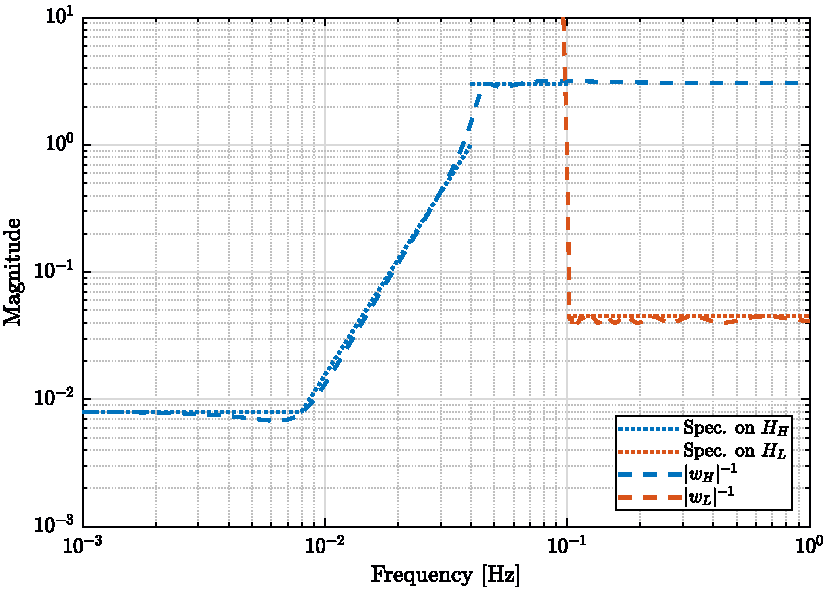
\includegraphics[width=\linewidth]{figs/ligo_weights.pdf}
  \end{tikzfigure}
  \vspace{-0.8em}
  \begin{tabular}{ll}
    \(\tikz[baseline=-0.5ex]{\draw[color=mycolor1, line width=1.5pt](0,0)--(1,0)}\) & {\small Custom designed \(7^{\text{th}}\) Order Transfer Function}\\
    \(\tikz[baseline=-0.5ex]{\draw[color=mycolor2, line width=1.5pt](0,0)--(1,0)}\) & {\small Type I Chebyshev Filter (Order \(20\))}\\
  \end{tabular}
\end{minipage}\hfill
\begin{minipage}[t]{0.5\linewidth}
  \vspace{-1.0em}
  \begin{tikzfigure}[Comparison of the FIR filters designed
    in \cite{hua05_low_ligo} (order 512) with the filters obtained with $\mathcal{H}_\infty$
    synthesis (order 27)]
    \label{fig:comp_fir_ligo_hinf}
    \centering
    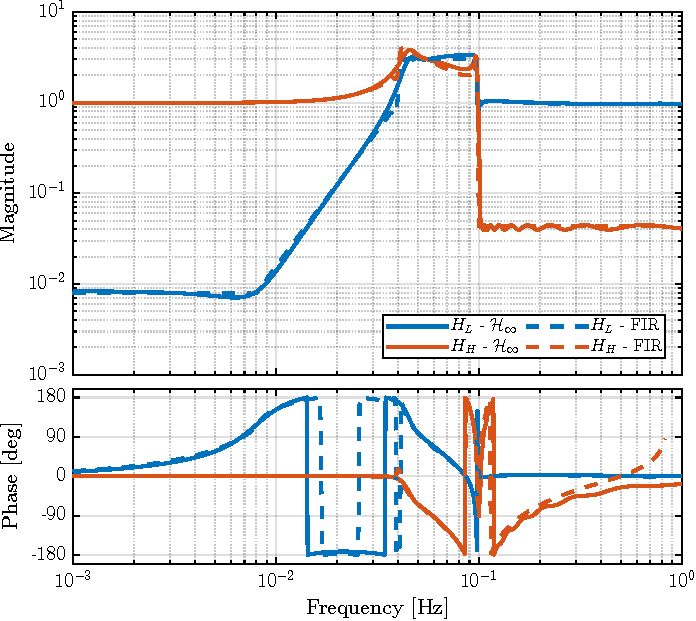
\includegraphics[width=\linewidth]{figs/comp_fir_ligo_hinf.pdf}
  \end{tikzfigure}
\end{minipage}

\bigskip

After synthesis, the obtained complementary filters are
compared with the FIR filters \cite{hua05_low_ligo} and are found
to be very close to each other (Fig.~\ref{fig:comp_fir_ligo_hinf}).